\documentclass[preprint,12pt]{article}

\usepackage{algorithmic}
\usepackage{algorithm}
\usepackage{enumerate}
\usepackage{enumitem}
\usepackage{graphics}
\usepackage{graphicx}
\usepackage{geometry}
\usepackage{amsmath}
\usepackage{wrapfig}
\usepackage{subfig}
\usepackage{framed}
\usepackage{color}
\usepackage{soul}
\usepackage{bm}

\usepackage{natbib}
\usepackage{multirow}
\usepackage[T1]{fontenc}
\usepackage[latin9]{inputenc}
%\usepackage{units}
\usepackage{esint}
\geometry{legalpaper,  margin=1in}

\newcommand{\CM}[2][green]{ {\sethlcolor{#1} \hl{#2}} }
\newcommand{\KB}[2][cyan]{ {\sethlcolor{#1} \hl{#2}} }
%THIS IS TO PUT ALL FLOATS AT THE END OF THE DOC SO THEY CAN BE SPLIT INTO A SEPARATE FILE
%%\usepackage{endfloat}
%\makeatother

%\usepackage{babel}

\begin{document}
\title{An Empirical Bayesian Framework for Assessing Partisan Bias in Redistricting Plans}

\author{Kevin Baas and Colin McAuliffe}

\maketitle


\section{Partisan Bias in the U.S. Congress 1972-2016\label{sec:Hist}}
We present an examination of partisan bias in the United States congress for elections from 1972 to 2016, which was collected by Brian Remlinger and Sam Wang \cite{Remliger_2017_}.
In order to obtain vote counts in uncontested races we use an imputation procedure.
The two party vote shares in an uncontested district are taken as the average of the vote shares for that district in the same cycle.
If a district is uncontested for an entire election cycle, then the vote share is taken to be equal to the average of the most partisan district for the winning party.
The voter turnout in the uncontested district is then taken as the average turnout in all contested elections in that state and election year.
Generally it is preferable to impute uncontested results using presidential results at the district level, but such data was not available for the entire time period under study.
Like all methods for examining gerrymandering, the specific asymmetry and the Bayesian simulation method are sensitive to the particular imputation technique employed, although a comprehensive study of this sensitivity is beyond the scope of our present work.

First, to illustrate the effect of asymmetry on the composition of congress, we compute the specific asymmetry for each state and election, and compare the Democratic popular vote share to the actual Democratic seat share as well as the Democratic seat share that would have resulted if each election had zero asymmetry.
This illustrates a few of the features of the specific asymmetry as a metric, but we note that this is not exactly representative of how the composition of congress would have been different had the proposed standard been enforced in each of these redistricting cycles.
The reason for this is that the proposed standard would enforce an expected asymmetry of zero, meaning on average no asymmetry would occur but in some elections asymmetry could occur by chance.
This result is shown in figure \ref{fig:AsymRemoved}, where it is evident that despite the natural multiplying effect of majoritarian elections, removing specific partisan asymmetry produces congressional representation closer to proportional with the popular vote, regardless of which party the net partisan asymmetry favors.  
Thus while proportionality of seats and votes is not enforced, gerrymandering tends to exacerbate and amplify the natural tendency of single winner elections to lead to disproportionate representation in favor of the majority party, and therefore removal of asymmetry caused by redistricting tends to lead to results that are closer to proportional.
If one were to use a metric that assumes votes should be proportional to seats, the 1970s would still be counted as gerrymandered, despite all partisan asymmetry being removed.  
Specific partisan asymmetry, however, never makes this error, while still leading to a substantial increase in the representativeness of congress as a whole.

\begin{figure}[htb!]
    \begin{center}
        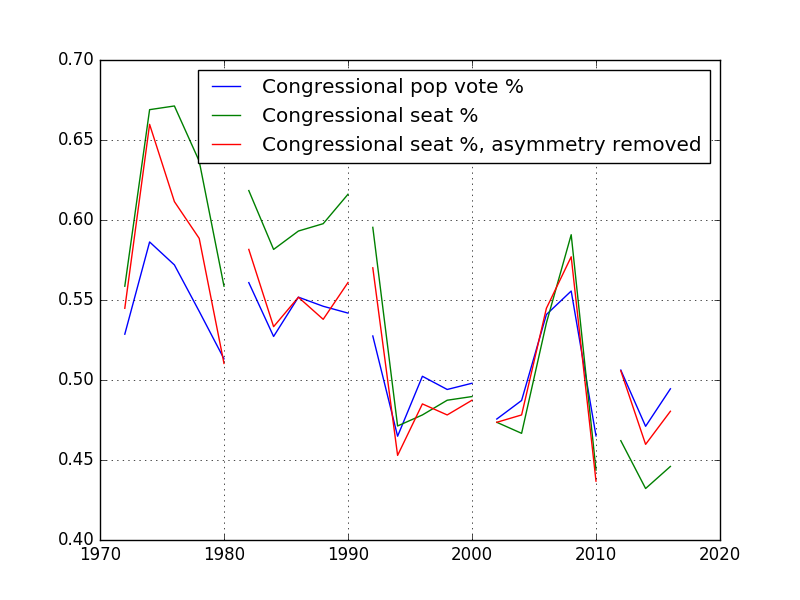
\includegraphics[scale=0.8]{../../Figures/HistoricAsymmetry/sv.png}
        \caption{Democratic vote share and seat share with asymmetry removed 1972-2016}\label{fig:AsymRemoved}
    \end{center}
\end{figure}

Next we account for random variability in the results by computing expected specific asymmetry for each state and redistricting cycle using 10,000 Monte Carlo samples.
First, we consider the net asymmetry, which is indicative of how gerrymandering may have affected the partisan composition of congress.
In figure \ref{fig:NetAsym}, the net observed asymmetry is shown for each election.
The expected net asymmetry for each redistricting cycle is also shown with 50\% and 90\% confidence intervals.
A progression is observed where the net asymmetry strongly favored Democrats in the 70's and 80's, mildly favored Democrats in the 90's, was roughly zero net asymmetry in the 2000's, and strongly favored Republicans in the 2010 cycle.
Histograms for the simulations can be found in figure \ref{fig:NetAsymHist}, which shows the expectation and variance of the net specific asymmetry.
In the 80's for example, Democrats could expect about 20 seats on average due to redistricting bias, with a negligibly small probability that the net national asymmetry would favor Republicans.
This situation has reversed entirely by the 2010 cycle, where Republicans can expect 18 seats on average due to redistricting bias.
Interestingly the 2000's show zero net bias on average, but this does not mean that the country was free of gerrymandering.
As we will show later in this section, there was significant gerrymandering by Republicans and Democrats in their respective territories, but the net effect of these gerrymanders tended to roughly cancel.
\begin{figure}[htb!]
    \begin{center}
        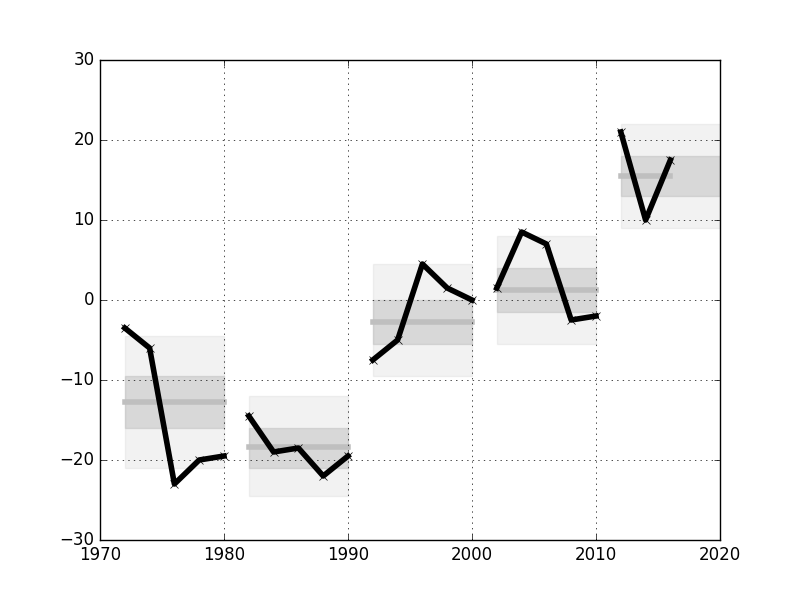
\includegraphics[scale=0.8]{../../Figures/ExpectedAsymmetry/netAsym.png}
        \caption{Net national asymmetry based on 10,000 simulations}\label{fig:NetAsym}
    \end{center}
\end{figure}
\begin{figure}[htb!]
    \begin{center}
        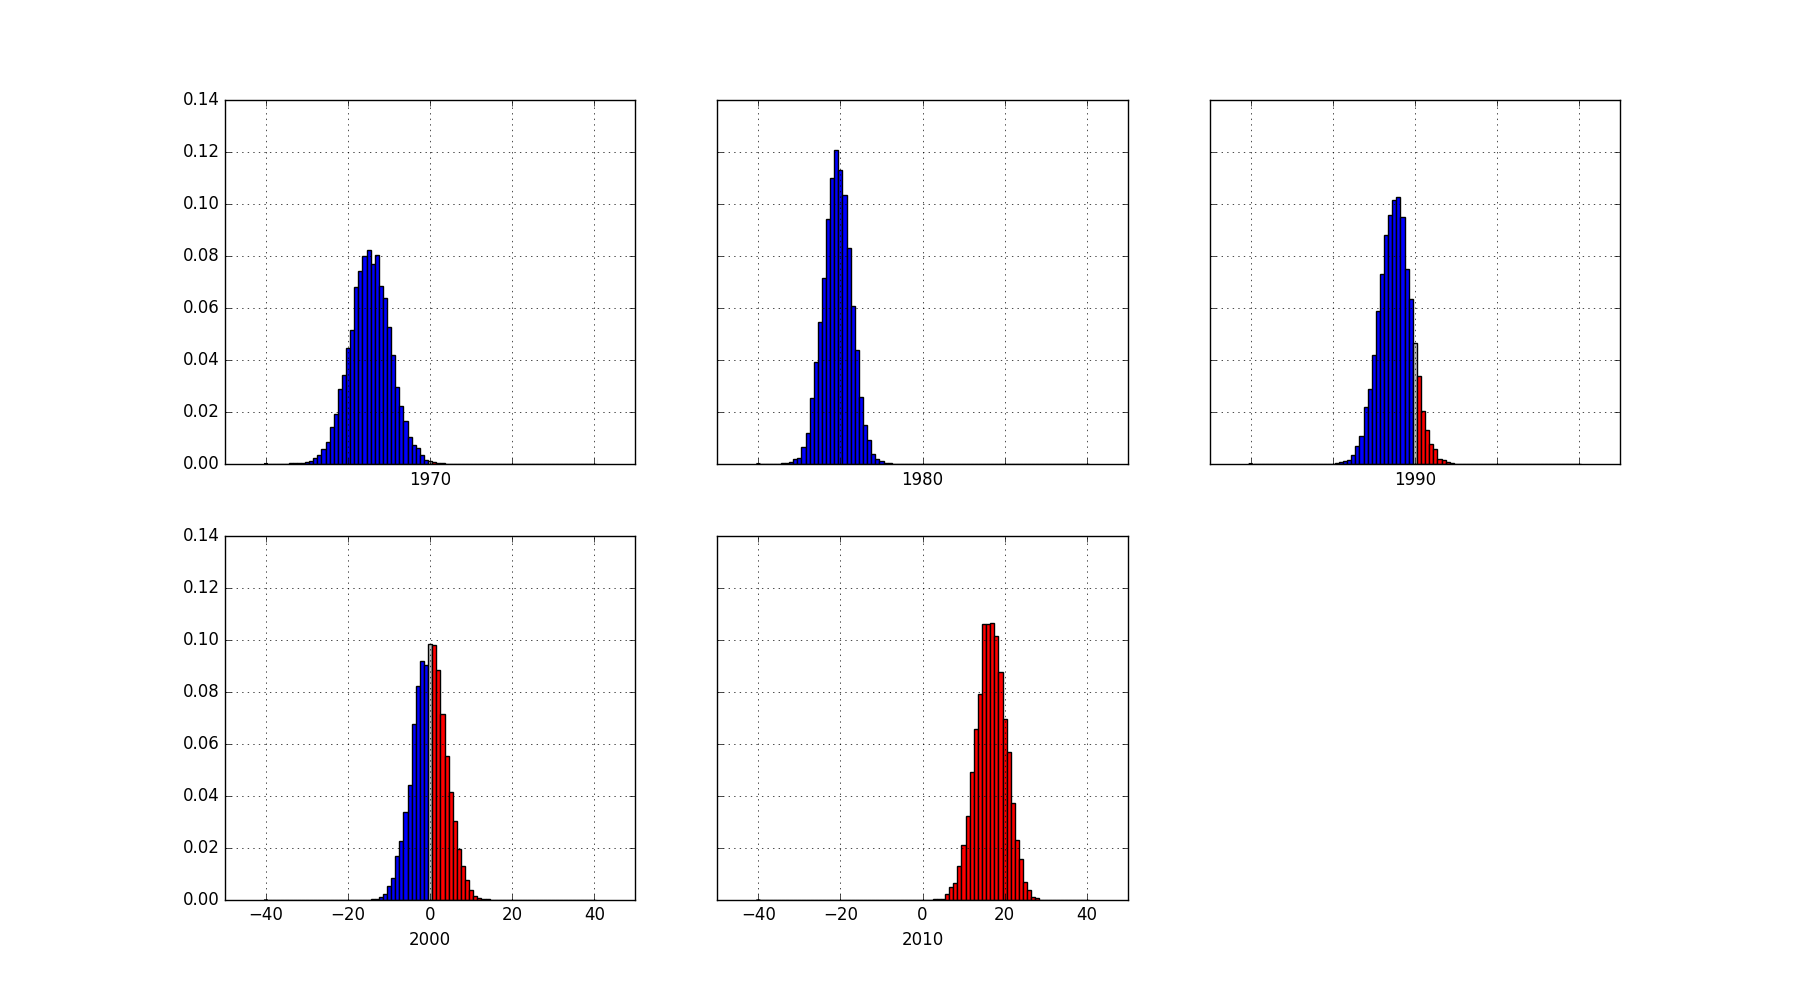
\includegraphics[scale=0.8]{../../Figures/ExpectedAsymmetry/netAsymHist.png}
        \caption{Net national asymmetry based on 10,000 simulations}\label{fig:NetAsymHist}
    \end{center}
\end{figure}

The results for the 2010s showing significant Republican gerrymandering are consistent with the well known REDMAP program, where Republicans lead a highly successful effort to gain control of several state houses in advance of the 2010 redistricting.
For earlier cycles, we observe qualitative agreement with a recent study covering the same time period \cite{Wang_2017_} in terms of which party benefited on net from gerrymandering.
Quantitatively, we observe some disagreement in terms of the magnitude of gerrymandering, with the present approach attributing more seats to redistricting bias.
This can be explained by differences in the analysis methodology.
The simulation technique employed in \cite{Wang_2017_} draws a 'fantasy' delegation from national voting results in order to determine if a party is winning seats excessively relative to its vote share\cite{Wang__}.
National voting results are used as a baseline, but this baseline itself will tend to change over time and may contain substantial bias, in which case only large gerrymanders will be successfully identified. 
Since the fantasy delegation technique draws a delegation from existing election results, the likelihood of a highly disproportionate outcome depends on the probability mass in the efficient win region for the party and cycle in question.
To verify this explanation for the differences arising from methodology, consider figure \ref{fig:meanHist}, which shows histograms of the average partisanship in each district and cycle.
There are differences from cycle to cycle in the probability mass in efficient win regions for each party, which arise from a number of causes including changes in redistricting bias.
In contrast, the present approach does not use a national baseline, and instead uses partisan asymmetry as the baseline to judge the effects of gerrymandering.
\begin{figure}[htb!]
    \begin{center}
        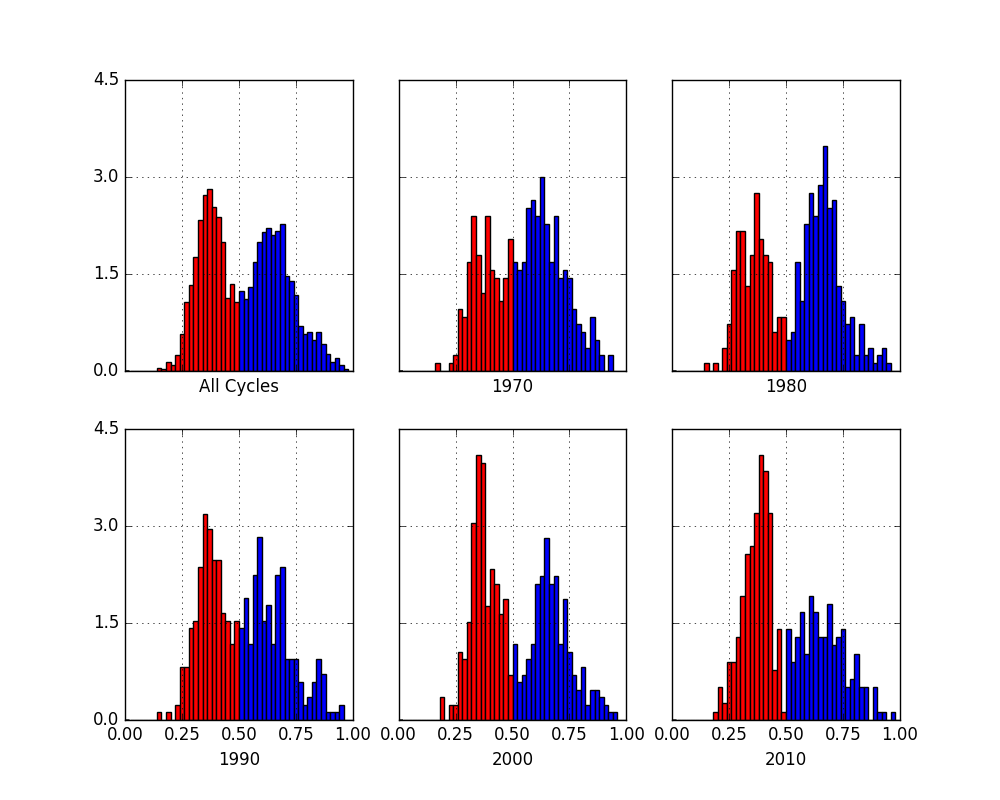
\includegraphics[scale=0.8]{../../Figures/HistoricAsymmetry/MeanHist.png}
        \caption{Distribution of mean district partisanship for each cycle}\label{fig:meanHist}
    \end{center}
\end{figure}

Differences in methodology aside, the result that the expected asymmetry favoring Democrats in the 80's is larger than that favoring Republicans in the 2010 cycle is surprising.
In the 2010 cycle, Republicans had the advantages of sophisticated redistricting algorithms, a high degree of geographic polarization, and low variability in voter preferences.
These factors enable effective gerrymandering and would not have been available to redistricters in the 80's.
On the other hand, Democrats controlled a significant number of states in the 80's and the national level of Democratic partisanship in congressional elections was fairly high, while it is closer to even in the 2010 cycle.
Compared to Republicans in the 2010 cycle, Democrats in the 80's obtained seats due to small levels of bias in a number of states, and additionally obtained significant numbers of seats in larger states like California and Texas.
Figure \ref{fig:80vs10} compares the simulated asymmetry distributions for California and Texas in the 80's and for Pennsylvania and North Carolina in the 2010's.
We can see that the variability of the asymmetry in Texas and California was higher than that of Pennsylvania and North Carolina.
It is also worth noting that the number of seats available in these states in the cycles under consideration.
In the 80's Texas has 24 seats and  California had 43, while in the in the 2010's, Pennsylvania had 18 seats and North Carolina had 13.
More district lines offers more opportunities for parties to manipulate redistricting to obtain a partisan advantage, and as a fraction of available seats, the gerrymanders in Pennsylvania and North Carolina are truly remarkable.
This is consistent with the fact that conditions and technology to produce highly stable gerrymanders would exist to a greater degree in the 2010s than in the 1980s.

\begin{figure}[htb!]
    \begin{center}
        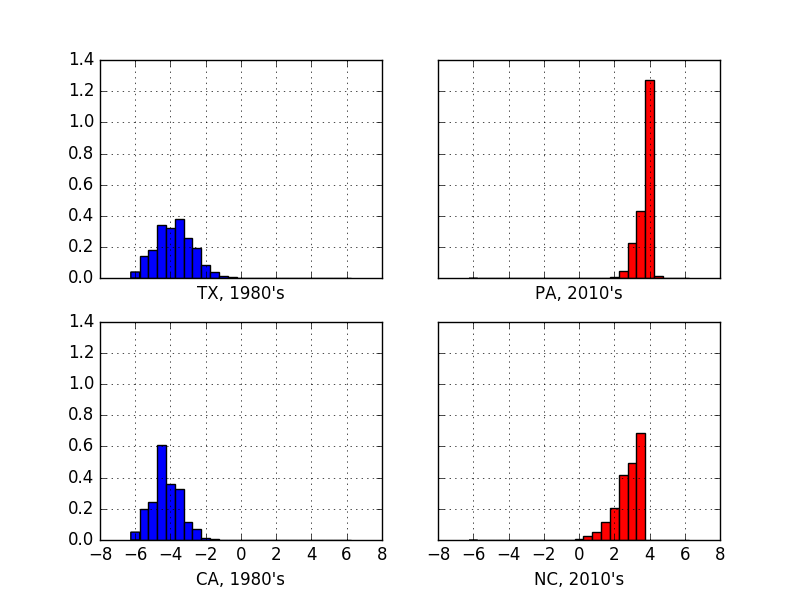
\includegraphics[scale=0.8]{../../Figures/ExpectedAsymmetry/80vs10.png}
        \caption{Histograms of the simulated asymmetries in Texas and California in the 1980's, and Pennsylvania and North Carolina in the 2010s}\label{fig:80vs10}
    \end{center}
\end{figure}

Net zero gerrymandering is preferable to a distorted congress, but net zero gerrymandering may still result in the congressional delegations of individual states being highly distorted.
We would therefore also like to examine the total asymmetry, or the sum of asymmetries in all states without regard to which party the asymmetry favors.
This tells us to what extent redistricting is being used to control election outcomes nationally.
This is plotted for each election cycle in \ref{fig:totalAsym}, where we observe that the total asymmetry has held fairly constant over each cycle.
Since there is a fixed number of seats available, every seat of partisan bias that redistrictors secure by gerrymandering is an equal amount of representation taken away from voters.
In other words, the relationship between voter representation and partisan bias resulting from redistricting is that of a zero-sum game: what one side gains, the other side loses.
Regardless of which party benefited from bias on balance, bias in redistricting appears to have affected the representation of millions of voters, for every congressional election since 1972.
\begin{figure}[htb!]
    \begin{center}
        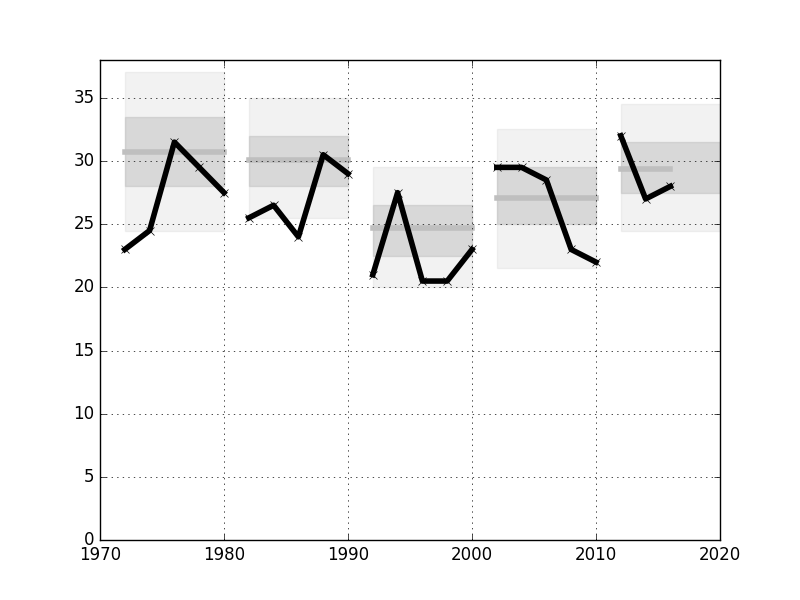
\includegraphics[scale=0.8]{../../Figures/ExpectedAsymmetry/totalAsym.png}
        \caption{Total national asymmetry based on 10,000 simulations}\label{fig:totalAsym}
    \end{center}
\end{figure}

While the total national asymmetry has held roughly constant over time, that is not to say that gerrymandering practices have held constant.
To the contrary, some aspects of the 2010 redistricting cycle are quite unprecedented.
Simultaneously, asymmetry has reduced in some states (at least in part due to redistricting reforms enacted in some of those states), while asymmetry has exploded in others.
States known to have been targeted by the REDMAP program are gerrymandered very aggressively in terms of the number of seats available and the level of partisanship in those states.
We can visualize how extreme the most aggressive gerrymanders are in each cycle are by sorting the expected asymmetry (as a percentage of available seats) in descending order for each state.
States with fewer than five seats are excluded since small asymmetries result as very large percentages.
This is shown in figure \ref{fig:asymRank}, where the 2010 cycle stands out as having three states with expected asymmetries that exceeded anything seen previously: Pennsylvania (18.4\%), North Carolina (18.0\%), and Georgia (14.1\%)
Following these are Virginia (11.9\%), Michigan (11.6\%), Ohio (11.1\%), and Wisconsin (10.2\%), which each have large asymmetries by historical standards.
All of these states showed a sudden increase in asymmetry in favor of Republicans after the 2010 redistricting, see table \ref{tab:Asym2000to2010} and figure \ref{fig:Asym2000to2010}. 
In contrast, California and New York had substantial asymmetries favoring Democrats in the 2000 cycle, and while they still show asymmetries favoring Democrats in the 2010 cycle, the magnitude of the asymmetry has decreased.
Previous cycles may have had moderate asymmetries in a larger number of states, but in terms of extreme gerrymandering, there has been no time since the Supreme Court ruled in \emph{Reynold v. Sims} (1964) that congressional districts must have roughly equal population, that is comparable to the 2010 cycle.

\begin{figure}[htb!]
    \begin{center}
        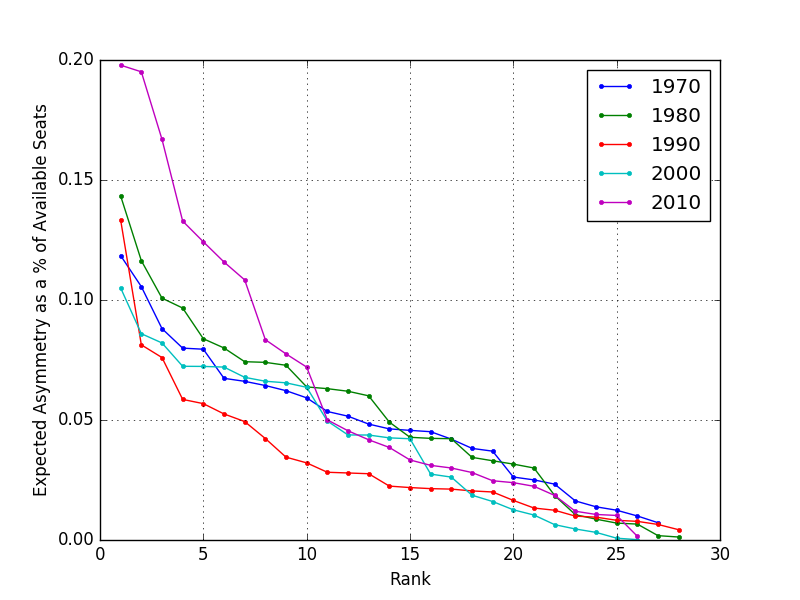
\includegraphics[scale=0.8]{../../Figures/ExpectedAsymmetry/asymRank.png}
        \caption{Expected asymmetry as a percentage of seats ranked in descending order for each redistricting cycle}\label{fig:asymRank}
    \end{center}
\end{figure}

\begin{table}[htb!]
\centering
\caption{Change in Expected Specific Asymmetry from 2000 to 2010 for states with large asymmetries in 2010 \label{tab:Asym2000to2010}}
\begin{tabular}{|l|l|l|l|}
\hline
State & Expected Specific     & Expected Specific & Net Change\\
      & Asymmetry, 2000 Cycle & Asymmetry, 2010 Cycle & \\
\hline
\hline
Pennsylvania & R 6.48\% & R 18.70\% & R 12.22\\
\hline
North Carolina & D 4.56\% & R 17.94\% & R 22.51\\
\hline
Georgia & R 3.74\% & R 16.22\% & R 12.48\\
\hline
Virginia & R 6.86\% & R 12.06\% & R 5.20\\
\hline
Michigan & R 6.53\% & R 11.63\% & R 5.10\\
\hline
Ohio & R 7.72\% & R 10.82\% & R 3.10\\
\hline
Wisconsin & D 2.01\% & R 9.90\% & R 11.91\\
\hline
California & D 8.48\% & D 2.17\% & R 6.31\\
\hline
New York & D 7.52\% & D 3.49\% & R 4.04\\
\hline
Illinois & R 0.83\% & D 2.96\% & D 3.79\\
\hline
\end{tabular}
\end{table}

\begin{figure}[htb!]
    \begin{center}
        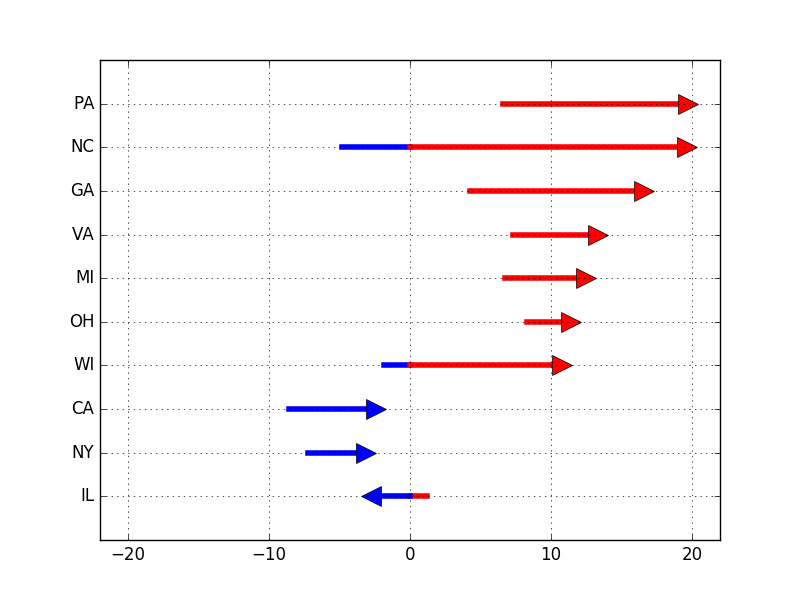
\includegraphics[scale=0.8]{../../Figures/ExpectedAsymmetry/diff2000to2010.png}
        \caption{Changes in the expected specific asymmetry from the 2000 redistricting cycle to the 2010 cycle. The arrow indicates the direction of the change in asymmetry.}\label{fig:Asym2000to2010}
    \end{center}
\end{figure}



\clearpage
\section*{Acknowledgment}
\section*{}
\bibliographystyle{unsrt}
\bibliography{gerrymandering}
\clearpage



\end{document}
